\documentclass[a4paper,11pt,notitlepage]{article}
\usepackage{sprawozdanie-ato}

\begin{document}


\title{\
Laboratorium Sieci Komputerowych\\\
Konfiguracja łącz i interfejsów sieciowych\
}
\author{\
Tomasz Cudziło, Barnaba Turek\\
\textsc{PW EE Informatyka}\\[6pt]
}
\date{\today}

\maketitle
\tableofcontents


\section{Cel ćwiczenia}

W ramach laboratorium mieliśmy za zadanie własnoręcznie skonfigurować i
przetestować kilka interfejsów sieciowych w systemie \bsd. Spośród dostępnych
łącz postanowiliśmy przetestować:

\begin{description}
    \item[łącze przewodowe \eth\textnormal{,}] które było dostępne na naszej
    stacji roboczej i podłączone fizycznie do sieci laboratorium, jednak nie
    było skonfigurowane na maszynie.
    \item[łącze radiowe \wifi\textnormal{,}] w ramach testowania którego,
    wypróbowaliśmy połączenie do punktu dostępowego --- \emph{access point}.
    \item[łącze radiowe \bt\textnormal{,}] dla którego połączyliśmy dwie
    maszyny laboratoryjne w układzie klient\dywiz serwer.
    \item[łącze szeregowe \rs\textnormal{,}] poprzez które połączyliśmy się
    z~konsolą maszyny \zielone{} za pomocą kabla szeregowego oraz za pomocą
    dwóch modemów \bt.
\end{description}


\section{Wykonanie ćwiczenia}

\subsection{\eth}
\label{sec:eth}

\subsubsection{Wprowadzenie}

W pierwszej części ćwiczenia skonfigurowano standardowe połączenie \eth. Jeden z
interfejsów był już skonfigurowany i udostępniał sprawne połączenie do
stacjonarnej sieci w laboratorium, ponieważ przez niego zabootowano system na
maszynie.

Sprawdzono, jakie interfejsy są dostępne.

\begin{lstlisting}
k9% ifconfig -a
sk0: flags=8843<UP,BROADCAST,RUNNING,SIMPLEX,MULTICAST> metric 0 mtu 1500
    options=80009<RXCSUM,VLAN_MTU,LINKSTATE>
    ether 00:11:d8:44:a4:37
    inet 194.29.146.189 netmask 255.255.255.0 broadcast 194.29.146.255
    media: Ethernet autoselect (100baseTX <full-duplex>)
    status: active
ipfw0: flags=8801<UP,SIMPLEX,MULTICAST> metric 0 mtu 65536
lo0: flags=8049<UP,LOOPBACK,RUNNING,MULTICAST> metric 0 mtu 16384
    options=3<RXCSUM,TXCSUM>
    inet 127.0.0.1 netmask 255.0.0.0
\end{lstlisting}

Do pracy z siecią skonfigurowany jest tylko interfejs \texttt{sk0}. Posiada już
pełną konfigurację na 3. wartwie OSI. Przynależy do sieci
\texttt{194.29.146.0/24}. Do tej sieci należy też maszyna \volt{} wykorzystując
swój interfejs \texttt{bge1}. Schemat opisanej konfiguracji znajduje się na
stronie \pageref{fig:eth:schemat-bez-konfiguracji}.

\begin{lstlisting}
volt% ifconfig -a
[...]
bge1: flags=8943<UP,BROADCAST,RUNNING,PROMISC,SIMPLEX,MULTICAST> metric 0 mtu 1500
    options=8009b<RXCSUM,TXCSUM,VLAN_MTU,VLAN_HWTAGGING,VLAN_HWCSUM,LINKSTATE>
    ether 00:e0:81:65:37:d4
    inet 194.29.146.3 netmask 255.255.255.0 broadcast 194.29.146.255
    inet 194.29.146.4 netmask 255.255.255.255 broadcast 194.29.146.4
    inet 194.29.146.11 netmask 255.255.255.255 broadcast 194.29.146.11
    media: Ethernet autoselect (1000baseT <full-duplex>)
    status: active
\end{lstlisting}

\begin{figure}[h!]
  \centering
  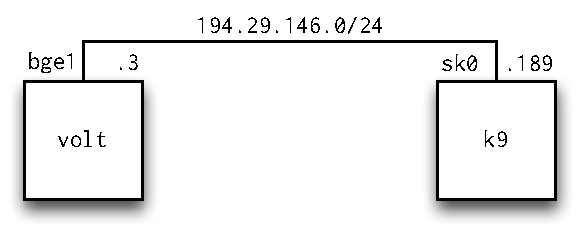
\includegraphics{figury/ethernet/schemat-bez-konfiguracji.pdf}
  \caption{Schemat początkowego połączenia \eth.}
  \label{fig:eth:schemat-bez-konfiguracji}
\end{figure}

Z wydruku \texttt{ifconfig -a} na \volt{}, w informacjach o interfejsie
\texttt{lagg0}, można wywnioskować obecność sieci \texttt{10.146.0.0/16}.

\begin{lstlisting}
volt% ifconfig lagg0
lagg0: flags=8943<UP,BROADCAST,RUNNING,PROMISC,SIMPLEX,MULTICAST> metric 0 mtu 9000
    options=9b<RXCSUM,TXCSUM,VLAN_MTU,VLAN_HWTAGGING,VLAN_HWCSUM>
    ether 00:1b:21:0d:e1:40
    inet 10.146.7.3 netmask 255.255.0.0 broadcast 10.146.255.255
    media: Ethernet autoselect
    status: active
    laggproto lacp
    laggport: em1 flags=1c<ACTIVE,COLLECTING,DISTRIBUTING>
    laggport: em0 flags=1c<ACTIVE,COLLECTING,DISTRIBUTING>
\end{lstlisting}

\subsubsection{Konfiguracja połączenia --- dodatkowy interfejs}
\label{sec:eth:konfiguracja}

W ramach ćwiczenia skonfigurowano dodatkowy interfejs na maszynie \kosiem{}
łączący ją z siecią \texttt{10.146.0.0/16}. Oczekiwany schemat połączeń znajduje
się na rys. \ref{fig:eth:schemat-po-konfiguracji}. Ponieważ przypisana nam
maszyna \kdziew{} nie była fizycznie podłączona do sieci, skorzystaliśmy zdalnie
z maszyny \kosiem.

\begin{figure}[h!]
  \centering
  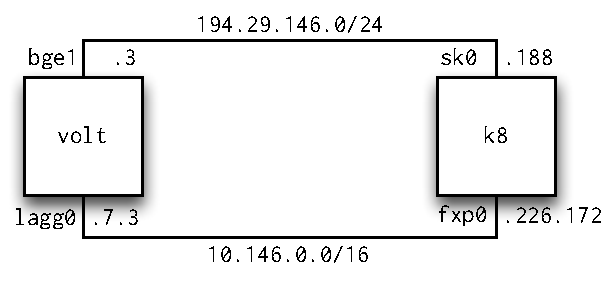
\includegraphics{figury/ethernet/schemat-po-konfiguracji.pdf}
  \caption{Schemat połączeń \eth{} po konfiguracji dodatkowego interfejsu na maszynie \kosiem.}
  \label{fig:eth:schemat-po-konfiguracji}
\end{figure}

Najpierw załadowano sterowniki do karty sieciowej firmy Intel. Nazwę modułu
znaleziono w instrukcji po wywołaniu skryptu \texttt{sterowniki -e}.

\begin{lstlisting}
k8% sudo kldload if_fxp
k8% ifconfig -a
[...]
fxp0: flags=8802<BROADCAST,SIMPLEX,MULTICAST> metric 0 mtu 1500
    options=2009<RXCSUM,VLAN_MTU,WOL_MAGIC>
    ether 00:d0:b7:0b:d2:fe
    media: Ethernet autoselect (100baseTX <full-duplex>)
    status: active
\end{lstlisting}

Po załadowaniu sterowników, zauważono powstanie nowego interfejsu o nazwie
\texttt{fxp0}. Użyliśmy programu \texttt{dhclient} by automatycznie
skonfigurować interfejs.

\begin{lstlisting}
k8% sudo dhclient fxp0
DHCPDISCOVER on fxp0 to 255.255.255.255 port 67 interval 6
DHCPDISCOVER on fxp0 to 255.255.255.255 port 67 interval 12
DHCPOFFER from 10.146.7.3
unknown dhcp option value 0xaf
DHCPREQUEST on fxp0 to 255.255.255.255 port 67
DHCPACK from 10.146.7.3
unknown dhcp option value 0xaf
bound to 10.146.226.172 -- renewal in 1800 seconds.

k8% ifconfig fxp0
fxp0: flags=8843<UP,BROADCAST,RUNNING,SIMPLEX,MULTICAST> metric 0 mtu 1500
    options=2009<RXCSUM,VLAN_MTU,WOL_MAGIC>
    ether 00:d0:b7:0b:d2:fe
    inet 10.146.226.172 netmask 255.255.0.0 broadcast 10.146.255.255
    media: Ethernet autoselect (100baseTX <full-duplex>)
    status: active

k8% netstat -r -f inet
Routing tables
Internet:
Destination        Gateway            Flags    Refs      Use  Netif Expire
default            gate               UGS         0        0    sk0
10.146.0.0         link#4             U           0        0   fxp0
10.146.226.172     link#4             UHS         0        0    lo0
localhost          link#3             UH          0        0    lo0
194.29.146.0       link#1             U           0    11770    sk0
k8.iem.pw.edu.pl   link#1             UHS         0        0    lo0
\end{lstlisting}

Widoczny jest proces nadawania adresu IP dla interfejsu. Adres został nadany
przez serwer DHCP z adresem \texttt{10.146.7.3}. Jest to adres \volt. Następnie
sprawdzono czy interfejs został skonfigurowany oraz czy tablice routingu zostały
odświeżone. Po sprawdzeniu konfiguracji przetestowano przepływ pakietów do
interfejsu. Z maszyny \volt{} wysłano 3 zapytania programem \texttt{ping}. Na
maszynie \kosiem{} programem \texttt{tcpdump} nasłuchiwano przychodzące pakiety
ICMP.

\begin{lstlisting}
# Z maszyny `volt` wysylano pakiety na adres przypisany
# maszynie `k8` przez serwer DHCP.
volt% ping -c 3 10.146.226.172
PING 10.146.226.172 (10.146.226.172): 56 data bytes
64 bytes from 10.146.226.172: icmp_seq=0 ttl=64 time=0.274 ms
64 bytes from 10.146.226.172: icmp_seq=1 ttl=64 time=0.249 ms
64 bytes from 10.146.226.172: icmp_seq=2 ttl=64 time=0.249 ms

--- 10.146.226.172 ping statistics ---
3 packets transmitted, 3 packets received, 0.0% packet loss
round-trip min/avg/max/stddev = 0.249/0.257/0.274/0.012 ms

# Na maszynie `k8` pakiety zostaly odebrane i odpowiedzi
# zostaly wyslane.
k8% sudo tcpdump -i fxp0 icmp
listening on fxp0, link-type EN10MB (Ethernet), capture size 65535 bytes
00:40:01.864733 IP 10.146.7.3 > 10.146.226.172: ICMP echo request, id 12044, seq 0, length 64
00:40:01.864766 IP 10.146.226.172 > 10.146.7.3: ICMP echo reply, id 12044, seq 0, length 64
00:40:02.866075 IP 10.146.7.3 > 10.146.226.172: ICMP echo request, id 12044, seq 1, length 64
00:40:02.866108 IP 10.146.226.172 > 10.146.7.3: ICMP echo reply, id 12044, seq 1, length 64
00:40:03.867117 IP 10.146.7.3 > 10.146.226.172: ICMP echo request, id 12044, seq 2, length 64
00:40:03.867146 IP 10.146.226.172 > 10.146.7.3: ICMP echo reply, id 12044, seq 2, length 64
^C
6 packets captured
63 packets received by filter
0 packets dropped by kernel
\end{lstlisting}

Konfiguracja przeszła testy pomyślnie. Dodatkowo nadano interfejsowi
\texttt{fxp0} drugi adres korzystając z opcji \texttt{alias} programu
\texttt{ifconfig}. By nie ryzykować zaburzenia pracy sieci jako drugi wybrano
adres z puli adresów sieci już skonfigurowanej tj. przypisano interfejsowi
\texttt{fxp0} statycznie adres \texttt{10.146.226.173/24}.

\begin{lstlisting}
k8% sudo ifconfig fxp0 alias 10.146.226.173/24
k8% ifconfig fxp0
fxp0: flags=8843<UP,BROADCAST,RUNNING,SIMPLEX,MULTICAST> metric 0 mtu 1500
    options=2009<RXCSUM,VLAN_MTU,WOL_MAGIC>
    ether 00:d0:b7:0b:d2:fe
    inet 10.146.226.172 netmask 255.255.0.0 broadcast 10.146.255.255
    inet 10.146.226.173 netmask 255.255.255.0 broadcast 10.146.226.255
    media: Ethernet autoselect (100baseTX <full-duplex>)
    status: active

k8% netstat -r
Routing tables
Internet:
Destination        Gateway            Flags    Refs      Use  Netif Expire
default            gate               UGS         0        0    sk0
10.146.0.0         link#4             U           0       11   fxp0
10.146.226.0       link#4             U           0        0   fxp0
10.146.226.172     link#4             UHS         0        0    lo0
10.146.226.173     link#4             UHS         0        0    lo0
localhost          link#3             UH          0        0    lo0
194.29.146.0       link#1             U           0    16644    sk0
k8.iem.pw.edu.pl   link#1             UHS         0        0    lo0
\end{lstlisting}

W tablicy routingu pojawiły się dwie nowe pozycje. Widać, że pakiety kierowane
do sieci \texttt{10.146.0.0/16} i \texttt{10.146.226.0/24} będą przechodziły
przez jeden interfejs.

Na koniec pracy z \eth{} usunięto konfigurację interfejsu \texttt{fxp0} i
odładowano sterowniki do karty sieciowej, z której interfejs korzystał.

\begin{lstlisting}
k8% sudo ifconfig fxp0 delete
k8% sudo kldunload if_fxp
k8% ifconfig fxp0
ifconfig: interface fxp0 does not exist
\end{lstlisting}

\subsection{\wifi}

\subsubsection{Wprowadzenie}

Pod terminem \wifi{} rozumiana jest sieć WLAN --- Wireless Local Area Network w
standardzie \texttt{IEEE 802.11}. W laboratorium urządzenia pracują zgodnie z
wersją \texttt{IEEE 802.11g} standardu. Standard zakłada pracę na paśmie
częstotliwości 2400 MHz \cite{wifi:pasmo} i oferuje szybkość do 54 Mbps
\cite{wifi:szybkosc} w zasięgu do 38 metrów od punktu dostępowego. W paśmie
standardu \texttt{g} mieści się 14 kanałów. W Polsce można używać kanały od 1.
do 13., czyli pasmo 2400 MHz do 2483,5 MHz. Przeczytano wstęp obsługi sieci
bezprzewodowych \cite{wifi:bsd-handbook} dla systemu \bsd{} i przystąpiono do
wykonania ćwiczenia.

Do maszyny \kdziew{} podłączone jest urządzenie \wifi{} przez port USB. By móc z
niego skorzystać postąpiono zgodnie z instrukcjami ze skryptu \texttt{sterowniki
-w}.

\begin{lstlisting}
k9% sudo kldload uhci ehci
k9% lsusb
[...]
ugen4.2: <Wireless-G ProtableUSB Adapter Cisco-Linksys> at usbus4, cfg=0 md=HOST spd=HIGH (480Mbps) pwr=ON
\end{lstlisting}

Po załadowaniu sterowników USB, urządzenie \wifi{} zostało wykryte przez system.
Załadowano sterowniki dla samego urządzenia \wifi{} i stwierdzono powstanie
nowego interfejsu o nazwie \texttt{ural0}.

\begin{lstlisting}
k9% sudo kldload if_ural
k9% ifconfig
[...]
ural0: flags=8802<BROADCAST,SIMPLEX,MULTICAST> metric 0 mtu 2290
    ether 00:12:17:60:ee:f8
    media: IEEE 802.11 Wireless Ethernet autoselect <adhoc> (autoselect <adhoc>)
    status: no carrier
\end{lstlisting}

Z tak załadowanym radiem \wifi{}, zaczęto konfigurować połączenie do sieci WLAN
\texttt{ZETiIS}.

\subsubsection{Konfiguracja połączenia --- do punktu dostępowego}

Stworzono pseudo\dywiz interfejs \texttt{wlan0}, który korzysta z rzeczywistego
interfejsu \texttt{ural0}. Nie podano specjalnego trybu pracy urządzenia,
zostaje wybrany tryb domyślny. Ustawiono polskie restrykcje dotyczące dostępnego
pasma i sprawdzono stan nowego interfejsu.

\begin{lstlisting}
k9% sudo ifconfig wlan0 create wlandev ural0
k9% sudo ifconfig wlan0 country PL
k9% ifconfig wlan0
wlan0: flags=8802<BROADCAST,SIMPLEX,MULTICAST> metric 0 mtu 1500
    ether 00:12:17:60:ee:f8
    media: IEEE 802.11 Wireless Ethernet autoselect (autoselect)
    status: no carrier
    ssid "" channel 1 (2412 MHz 11b)
    regdomain ETSI country PL authmode OPEN privacy OFF txpower 30
    bmiss 7 scanvalid 60 bgscan bgscanintvl 300 bgscanidle 250 roam:rssi 7
    roam:rate 1 bintval 0
\end{lstlisting}

Uruchomiono interfejs \texttt{wlan0} oraz przeszukano dostępne sieci \wifi.

\begin{lstlisting}
k9% sudo ifconfig wlan0 up
k9% sudo ifconfig wlan0 scan
SSID/MESH ID    BSSID              CHAN RATE   S:N     INT CAPS
[...]
ZETiIS          00:1e:52:79:ca:59    6   54M -74:-95  100 EPS  RSN HTCAP WME
pwwifi-stud...  00:24:14:31:95:03   11   54M -87:-95  102 ES   HTCAP WME
pwwifi-stud...  00:21:a0:81:86:c3    1   54M -83:-95  102 ES   HTCAP WME
pwwifi          00:24:14:31:95:00   11   54M -87:-95  102 ES   HTCAP WME
pwwifi          00:21:a0:0f:e2:40   11   54M -88:-95  102 ES   HTCAP WME
\end{lstlisting}

Razem z listą innych sieci, widoczna jest sieć \texttt{ZETiIS} z atrybutami
\texttt{EPS}. Każdy ze znaków informuje o danej cesze sieci. Interesujące nas
cechy to:

\begin{description}
    \item[E] --- aktualny nadajnik jest częścią większej infrastruktury, nie
        pracuje w trybie ad\dywiz hoc,
    \item[P] --- sieć wymaga autoryzacji użytkownika. Dla porównania widać, że
        sieć \texttt{pwwifi} nie jest zabezpieczona na tej warstwie.
\end{description}

Podano jawną nazwę sieci, do której chcemy się połączyć. Nie uzyskano
połączenia. Niezbędny jest sekret uprawniający do skorzystania z sieci.

\begin{lstlisting}
k9% sudo ifconfig wlan0 ssid ZETiIS
k9% sudo ifconfig wlan0
wlan0: flags=8843<UP,BROADCAST,RUNNING,SIMPLEX,MULTICAST> metric 0 mtu 1500
    ether 00:12:17:60:ee:f8
    media: IEEE 802.11 Wireless Ethernet autoselect (autoselect)
    status: no carrier
    ssid ZETiIS channel 11 (2462 MHz 11g)
    regdomain ETSI country PL authmode WPA2/802.11i privacy OFF
    txpower 30 bmiss 7 scanvalid 60 bgscan bgscanintvl 300 bgscanidle 250
    roam:rssi 7 roam:rate 5 protmode CTS bintval 102
\end{lstlisting}

Ponieważ sieć \texttt{ZETiIS} korzysta z szyfrowania WPA w wersji korporacyjnej,
potrzebne są dane autoryzujące użytkownika, oraz wymiana kluczy i szyfrowanie,
czym zajmuje się usługa \texttt{wpa\_supplicant}. Włączono demona
\texttt{wpa\_supplicant} dla interfejsu \texttt{wlan0}, podano sekret
użytkownika i nawiązano połączenie z siecią.

\begin{lstlisting}
k9% sudo service wpa_supplicant start wlan0
Starting wpa_supplicant.

k9% sudo wpa_cli ping
PONG

k9% sudo wpa_cli status
wpa_state=DISCONNECTED
Supplicant PAE state=DISCONNECTED
suppPortStatus=Unauthorized
EAP state=DISABLED
selectedMethod=25 (EAP-PEAP)
EAP TLS cipher=DHE-RSA-AES256-SHA
EAP-PEAPv0 Phase2 method=MSCHAPV2

k9% sudo wpa_cli identity ZETiIS cudzilot
OK

k9% sudo wpa_cli password ZETiIS haslo12345
OK

k9% sudo wpa_cli select_network ZETiIS
OK

k9% sudo wpa_cli status
bssid=00:1e:52:79:ca:59
ssid=ZETiIS
id=0
mode=station
pairwise_cipher=CCMP
group_cipher=CCMP
key_mgmt=WPA2/IEEE 802.1X/EAP
wpa_state=COMPLETED
Supplicant PAE state=AUTHENTICATED
suppPortStatus=Authorized
EAP state=SUCCESS
selectedMethod=25 (EAP-PEAP)
EAP TLS cipher=DHE-RSA-AES256-SHA
EAP-PEAPv0 Phase2 method=MSCHAPV2

k9% sudo ifconfig wlan0
wlan0: flags=8843<UP,BROADCAST,RUNNING,SIMPLEX,MULTICAST> metric 0 mtu 1500
    ether 00:12:17:60:ee:f8
    media: IEEE 802.11 Wireless Ethernet DS/1Mbps mode 11g
    status: associated
    ssid ZETiIS channel 6 (2437 MHz 11g) bssid 00:1e:52:79:ca:59
    regdomain ETSI country PL authmode WPA2/802.11i privacy ON
    deftxkey UNDEF AES-CCM 3:128-bit txpower 30 bmiss 7 scanvalid 450
    bgscan bgscanintvl 300 bgscanidle 250 roam:rssi 7 roam:rate 5
    protmode CTS roaming MANUAL
\end{lstlisting}

Następnie skonfigurowano warstwę 3. dla interfejsu \texttt{wlan0}, za pomocą
DHCP. Analogicznie do konfiguracji z sekcji \ref{sec:eth:konfiguracja}. Łącze
przetestowano wysyłając zapytania z \volt{} i nasłuchując ruch na interfejsie.

\begin{lstlisting}
k9% sudo dhclient wlan0
DHCPDISCOVER on wlan0 to 255.255.255.255 port 67 interval 4
DHCPDISCOVER on wlan0 to 255.255.255.255 port 67 interval 9
DHCPOFFER from 10.146.7.3
unknown dhcp option value 0xaf
DHCPREQUEST on wlan0 to 255.255.255.255 port 67
DHCPACK from 10.146.7.3
unknown dhcp option value 0xaf
bound to 10.146.226.113 -- renewal in 1800 seconds.

volt% ping -c 1 10.146.226.113
PING 10.146.226.113 (10.146.226.113): 56 data bytes
64 bytes from 10.146.226.113: icmp_seq=0 ttl=64 time=2.822 ms
--- 10.146.226.113 ping statistics ---
1 packets transmitted, 1 packets received, 0.0% packet loss
round-trip min/avg/max/stddev = 2.822/2.822/2.822/0.000 ms

k9% sudo tcpdump -i wlan0 icmp
tcpdump: verbose output suppressed, use -v or -vv for full protocol decode
listening on wlan0, link-type EN10MB (Ethernet), capture size 65535 bytes
00:35:53.738249 IP 10.146.7.3 > 10.146.226.113: ICMP echo request, id 22633, seq 0, length 64
00:35:53.738287 IP 10.146.226.113 > 10.146.7.3: ICMP echo reply, id 22633, seq 0, length 64
^C
2 packets captured
259 packets received by filter
0 packets dropped by kernel
\end{lstlisting}

Na koniec ćwiczenia zatrzymano demon \texttt{wpa\_supplicant} i usunięto
pseudo\dywiz interfejs \texttt{wlan0}.

\begin{lstlisting}
k9% sudo service wpa_supplicant stop wlan0
Stopping wpa_supplicant.
Waiting for PIDS: 1275.
k9% sudo ifconfig wlan0 destroy
\end{lstlisting}

%\subsubsection{Konfiguracja połączenia --- tryb ad\dywiz hoc}

\section{bluetooth}
\label{sec:bt}
\subsection{Wprowadzenie}
Bluetooth to własnościowy standard komunikacji bezprzewodowej.

Korzystając z~połączenia Bluetooth możliwe jest tworzenie sieci \texttt{PAN} - Personal Area Network.

Sieci \texttt{PAN} oparte o~bluetooth pozwalają na połączenie maksymalnie 8 urządzeń w~konfiguracji klienci\dywiz serwer\cite{wiki:pan}.
W~sieci występuje jeden serwer i~wszyscy klienci powinni znajdować się w~jego zasięgu.

Możliwe jest także zwiększenie zasięgu sieci poprzez węzły pośrednie (tzw. \emph{scatternet})\cite{bt}.
\begin{figure}[h]
  \centering
  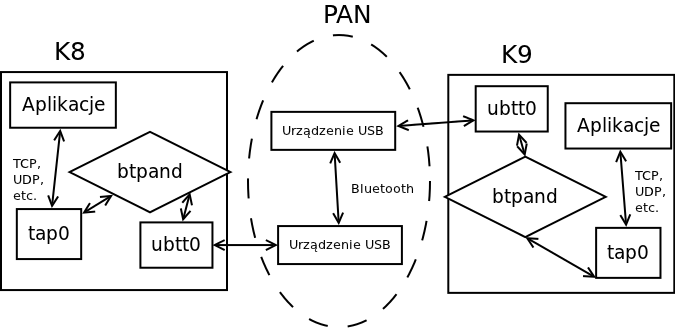
\includegraphics[width=\textwidth]{figury/schemat-bluetooth.png}
  \caption{Schemat ideowy}
\end{figure}

W systemie FreeBSD na którym mamy zajęcia połączenia w tej technologii można realizować za pomocą wirtualnego urządzenia \texttt{TAP}, na które demon \texttt{btpand} przekierowuje pakiety.

\subsection{Przebieg ćwiczenia}
Po zalogowaniu się na maszynę laboratoryjną załadowaliśmy niezbędne sterowniki (zgodnie z~instrukcjami podanymi przez skrypt \texttt{sterowniki -b}: \texttt{uhci, ehci, ng\_ubt}.
Są to sterowniki odpowiedzialne za stos \texttt{USB} oraz samo urządzenie bluetooth (podłączone do komputera przez \texttt{USB}).

Po załadowaniu sterowników musieliśmy odłączyć i~podłączyć urządzenie, żeby zostało wykryte.

\begin{lstlisting}[caption={Sprawdzenie, że urządzenie zostało wykryte}]
$ dmesg | tail
ugen4.2: <ZyDAS> at usbus4
ugen1.2: <Logitech> at usbus1
ugen0.2: <vendor 0x0a12> at usbus0^
ubt0: <vendor 0x0a12 product 0x0001, class 224/1, rev 1.10/3.73, addr 2> on usbus0
\end{lstlisting}

Kiedy upewniliśmy się, ze urządzenie zostało poprawnie rozpoznane, zgodnie z~instrukcją uruchomiliśmy usługę \texttt{bluetooth}.
\begin{lstlisting}[caption={Sprawdzenie, że urządzenie zostało wykryte}]
$ sudo service bluetooth onestart ubt0
\end{lstlisting}
Polecenie to nie uruchamia żadnego systemowego demona, ale konfiguruje urządzenie bluetooth do pracy, za pomocą komend \texttt{ngctl} i~\texttt{hccontrol}.

Polecenie \texttt{ngctl} służy do tworzenia i~wysyłania komand do węzła \emph{netgraph}.
\emph{Netgraph} to podsystem jądra, który pozwala obsługiwać różne interfejsy (L2TP, PPTP, ATM, bluetooth). Pozwala modularnie implementować protokoły (niezależnie od urządzeń) i~zapewnia spójny system komend dla różnych protokłów i~urządzeń\cite{man:netgraph}.

Polecenie \texttt{hccontroll} zapewnia obsługę komend specyficznych dla interfejsów \emph{Bluetooth}.

Następnie połączyliśmy się za pomocą bluetooth z~maszyną \textbf{k8}:
\begin{lstlisting}[caption={Połączenie na poziomie protokołu bluetooth}]
$ hccontrol read_bd_addr #k8
BD_ADDR: 00:08:1b:00:d3:3a

# adresy urzadzen beda potrzebne do zestawienia sieci PAN
# i pozwalaja sprawdzicz, czy urzadzenie zostalo poprawnie zainicjowane
# w podsystemie netgraph.

$ hccontrol read_bd_addr #k9
BD_ADDR: 00:08:1b:00:2e:e3

# sprawdzamy, czy 'widzimy' docelowe urzadzenie

$ sudo hccontrol inquiry
[...]
Inquiry result, num_responses=1
Inquiry result #0
  BD_ADDR: F4
  Page Scan Rep. Mode: 0x1
  Page Scan Period Mode: 0x2
  Page Scan Mode: 00
  Class: 00:1f:00
  Clock offset: 0x66c4
[...]
Inquiry complete. Status: No error [00]

# sprawdzamy czy mozemy sie z nim komunikowac

$ l2ping -a 00:08:1b:00:d3:3a
44 bytes from K8 seq_no=1 time=26.587 ms result=0
44 bytes from K8 seq_no=2 time=22.212 ms result=0
44 bytes from K8 seq_no=3 time=29.836 ms result=0
44 bytes from K8 seq_no=4 time=39.968 ms result=0
44 bytes from K8 seq_no=5 time=20.572 ms result=0

# tworzymy siec pan (skrypt bt-pan uruchamia demona btpand)

$ sudo bt-pan -c 00:08:1b:00:d3:3a # utworzenie sieci pan z k8 w roli serwera

BD_ADDR: 00:08:1b:00:2e:e3
00:08:1b:00:2e:e3Starting sdpd.
btpand[1429]: Searching for NAP service at 00:08:1b:00:d3:3a
btpand[1429]: Found PSM 15 for service NAP
btpand[1429]: Opening connection to service 0x1116 at 00:08:1b:00:d3:3a
btpand[1429]: channel_open: (fd#4)
btpand[1429]: Using interface tap0 with addr 00:00:1b:00:2e:e3
btpand[1429]: channel_open: (fd#5)
skonfiguruj teraz interfejs tap0   np. ifconfig tap0 10.9
\end{lstlisting}

Skrypt bt-pan nie tylko połączył nas z urządzeniem bluetooth komputera \textbf{k8}, ale też utworzył wirtualny interfejs sieciowy.
Stworzony przez ten skrypt interfejs jest powiazany z konkretną siecią PAN.

Demon \texttt{btpand} opakowuje wychodzące pakiety wyższych warstw modelu OSI w~ramki protokołu Bluetooth Network Encapsulation Protocol (BNEP).
Protokół BNEP wspiera te same protokoły sieciowe, które wspiera IEEE 802.3/Ethernet\cite[bnep].

Demon \texttt{btpand} zapewnia przekierowanie pakietów \emph{ethernetowych} przychodzących na urządzenie Bluetooth na wirtualny interfejs (w~naszym przypadku \texttt{tap0}).

Uruchomił także demona \emph{sdpd}, który pozwala udostępniać usługi za pomocą bluetooth i~wyszukiwać usługi na innych urządzeniach.

Następnym krokiem było, zgodnie z~instrukcjami polecenia skryptu \texttt{bt-pan} skonfigurowaniu interfejsu tap0.
(A~także wykonanie analogicznych poleceń na maszynie k8).

\begin{lstlisting}[caption={Skonfigurowanie interfejsów zgodnie z~protokołem IP}]
$ sudo ifconfig tap0 10.8
$ ifconfig

[...]

tap0: flags=8843<UP,BROADCAST,RUNNING,SIMPLEX,MULTICAST> metric 0 mtu 1500
  options=80000<LINKSTATE>
  ether 00:08:1b:00:2e:e3
  inet 10.0.0.9 netmask 255.0.0.0 broadcast 10.255.255.255
  Opened by PID 1429

$ ping 10.8

64 bytes from 10.0.0.8: icmp_seq=0 ttl=64 time=68.957 ms
[...]

# wygenerowalismy ruch TCP na interfejsach korzystajac z polecenia netcat

$ sudo tcpdump -i tap0 host 10.8 tcp
tcpdump: verbose output suppressed, use -v or -vv for full protocol decode
listening on tap0, link-type EN10MB (Ethernet), capture size 65535 bytes
17:02:34.236847 IP 10.0.0.8.11342 > 10.0.0.9.1337: Flags [P.], seq 982177280:982177281, ack 3979280866, win 1040, options [nop,nop,TS val 13104042 ecr 1310253008], length 1
17:02:34.336347 IP 10.0.0.9.1337 > 10.0.0.8.11342: Flags [.], ack 1, win 1040, options [nop,nop,TS val 1310280520 ecr 13104042], length 0
17:02:34.777801 IP 10.0.0.8.11342 > 10.0.0.9.1337: Flags [P.], seq 1:2, ack 1, win 1040, options [nop,nop,TS val 13104579 ecr 1310280520], length 1
17:02:34.877216 IP 10.0.0.9.1337 > 10.0.0.8.11342: Flags [.], ack 2, win 1040, options [nop,nop,TS val 1310281061 ecr 13104579], length 0

\end{lstlisting}


\subsection{Połączenie szeregowe}

\subsubsection{Wprowadzenie}

Systemy z~rodziny *NIX pozwalają na korzystanie z~konsoli za pośrednictwem portu
szeregowego (zwykle rs\dywiz 232). Funkcja ta jest przydatna zarówno dla
administratorów (ponieważ nie trzeba podłączać klawiatury i~monitora do serwera)
jak i~programistów, pracujących nad sterownikami.

Skorzystaliśmy z~konsoli aby połączyć się z~urządzeniem \zielone{} z maszyny
\kdziew. Do zestawienia takiego połączenia za pomocą portu szeregowego potrzebny
jest kabel typu \emph{null\dywiz modem}\cite{serial-console}.

\subsubsection{Konfiguracja połączenia --- null\dywiz modem}
\label{sec:serial:null-modem}

Po załadowaniu niezbędnych sterowników i~podłączeniu kabla \emph{null\dywiz
modem} zajrzeliśmy do pliku \texttt{/etc/remote}, w~którym zdefiniowane są
systemy rozpoznawalne przez program \texttt{tip}. Dla każdego systemu podana
jest nazwa urządzenia oraz konfiguracja połączenia, gdzie ustalane są m.in. typ
kontroli parzystości i~prędkość transmisji.

\begin{lstlisting}[caption={Linie z \texttt{/etc/remote} dotyczące naszego połączenia.}]
modem:dv=/dev/cuau0:br#115200:pa=none:
ps:dv=/dev/cuau0:br#115200:pa=none:
bt:dv=/dev/ttyp0:br#115200:pa=none:
\end{lstlisting}

Skorzystaliśmy z~urządzenia \texttt{ps}, ponieważ instrukcja ze skryptu
\texttt{sterowniki~-s} sugerowała połączenie wykorzystujące urządzenie
\texttt{/dev/cuau0}. Dodatkowo zadeklarowana w \texttt{/etc/remote} prędkość
transmisji zgadzała się z prędkością zaproponowaną w instrukcji.

\begin{lstlisting}[caption={Połączenie z konsolą maszyny \zielone{} za pomocą programu \texttt{tip}.}]
k9% sudo tip ps
^Gconnected

Login incorrect
debian login:
debian login: +++RESET

POST: 012345689bcefghips1234ajklnopqr,,,tvwxy

comBIOS ver. 1.33c 20080626  Copyright (C) 2000-2008 Soekris Engineering.
\end{lstlisting}

Żeby zrestartować maszynę \zielone{} zastosowaliśmy polecenie z zestawu rozkazów
Hayesa tj. wpisaliśmy \texttt{+++} i po odczekaniu chwili wydaliśmy polecenie
\texttt{RESET}. Następnie z pomocą prowadzącego uruchomiliśmy na \zielone{}
system \bsd.

\subsubsection{Konfiguracja połączenia --- \bt}

Dzięki zastosowaniu modemu radiowego Firefly możliwe jest bezprzewodowe
połączenie z~konsolą. Modem Firefly posiada tryb pracy, w~którym w~przezroczysty
sposób zastępuje kabel szeregowy, jednak wymagane są dwa modemy na każde
połączenie.

Zamiast tego w~laboratorium każda z~maszyn Soekris ma podpięty jeden modem,
a~komputery\dywiz terminale łączą się z tym modemem za pomocą własnego,
niespecjalizowanego radia \bt. Rozwiązanie takie pozwala ograniczyć liczbę
potrzebnych modemów Firefly, wymaga jednak więcej konfiguracji.

Po załadowaniu niezbędnych sterowników i~wyszukaniu interesujących nas urządzeń
w~eterze (analogicznie do ćwiczenia \ref{sec:bt}), próbowaliśmy skorzystać ze
skryptu \texttt{bt-spp}. Niestety skrypt aktualnie nie daje oczekiwanych
rezultatów.

Wykryliśmy, że problem dotyczy tworzenia nowego terminala przez polecenie
\texttt{rfcomm\_sppd}. Wyłączenie tej funkcjonalności ograniczyłoby zastosowania
skryptu \texttt{bt-spp}, ale na nasze potrzeby było wystarczające. Usunęliśmy ze
skryptu komendę tworzącą urządzenie pełniące rolę pseudo\dywiz terminala. W
efekcie konsola, z~którą chcemy się połączyć jest dostępna w~konsoli, z~której
się łączyliśmy, analogicznie do działania programu \texttt{tip} w~sekcji
\ref{sec:serial:null-modem}.

\begin{lstlisting}[caption={Połączenie z konsolą maszyny Soekris za pomocą programu \texttt{rfcomm\_sppd}.}]
# Na maszynie k9.
k9% hostname
k9

# Laczymy sie z maszyna Soekris poprzez modem Firefly.
k9% rfcomm_sppd -a F11
rfcomm_sppd[1656]: Starting on stdin/stdout...
Login:stud
Password:zetis

Last login: Fri Apr 13 04:57:21 on ttyu0
FreeBSD 9.0-STABLE (SOEKRIS) #0 r233366M: Sat Mar 24 00:57:52 CET 2012

# Jestesmy w konsoli maszyny Soekris.
so4801% hostname
so4801
\end{lstlisting}



\section{Wnioski i spostrzeżenia}


\begin{thebibliography}{9}
    \bibitem{serial-console}
        \url{http://www.freebsd.org/doc/en_US.ISO8859-1/books/handbook/serialconsole-setup.html}
    \bibitem{wiki:pan}
        \url{http://en.wikipedia.org/wiki/Personal_area_network}
    \bibitem{bt}
        \url{http://progtutorials.tripod.com/Bluetooth_Technology.htm}
    \bibitem{bnep}
        \url{http://grouper.ieee.org/groups/802/15/Bluetooth/BNEP.pdf}
    \bibitem{man:netgraph}
        {\texttt{man (4) netgraph}}
    \bibitem{man:remote}
        {\texttt{man (5) netgraph}}
\end{thebibliography}

\end{document}
